\chapter{No-name yet}

\newpage

\section{Query taxonomy and re-usability formalization}

This section presents the description and formalization of the different types of queries which \textit{(i)} can be processed by our integration approach; and \textit{(ii)} can be compared to previous integration requests in order to take advantage from previous integration plans. The query definition is introduced below.

\begin{definition}
A query is defined as a $n$-tuple:
%
\begin{center}
$Q := \langle A, R, S, C, w  \rangle$
\end{center}
%
where: $A$ is a set of abstract services defining the query $Q$;
$R$ is a set of user preferences that can be defined over the data services or the entire query;
$S$ is a set of data services that were selected satisfying the restrictions defined by $R$ to potentially rewrite the query $Q$;
$C$ is a set of compositions that were produced using the data services in $S$ and satisfying the restrictions defined by $R$ that potentially can answer the query $Q$; and
$w$ is the composition that were selected and executed to answer the query $Q$. 
\end{definition}

The query taxonomy proposed below is defined according to the type of relation that can be established between two queries. 
Queries are classified in four groups: 
\begin{itemize}
\item \textit{Group 1:} The data denoted by the answer of $Q_{1}$ is the same data expected by the answer of $Q_{2}$. For example, $Q_{1}$ and $Q_{2}$ retrieve patients that were infected by pneumonia.
\item \textit{Group 2:} The data denoted by the answer of $Q_{1}$ is a subset of the data denoted by the answer of $Q_{2}$. For example, $Q_{2}$ retrieves patients that were infected by pneumonia and $Q_{1}$ retrieves patients that were infected by pneumonia and treated by the doctor Lucas.
\item \textit{Group 3:} The data denoted by the answer of $Q_{1}$ is a superset of the data denoted by the answer of $Q_{2}$. For example, $Q_{2}$ retrieves patients that were infected by pneumonia and treated by the doctor Lucas, and $Q_{1}$ retrieves patients that were infected by pneumonia.
\item \textit{Group 4:} The data denoted by the answer of $Q_{1}$ is different of the data denoted by the answer of $Q_{2}$. For example, $Q_{2}$ retrieves patients that were infected by pneumonia and treated by the doctor Lucas, and $Q_{1}$ retrieves patients that were infected by pneumonia with admission in the hospital Edouard Herriot.
\end{itemize}

To understand the different types of query, basic concepts regarding \textit{(i)} user requirements, \textit{(ii)} requirements domain, \textit{(iii)} requirements evaluation and \textit{(iv)} comparable requirements should be introduced:

\begin{definition}
An user requirement $r$ is in the form $x \otimes c$, where $x$ is an identifier; $c$ is a constant; and $\otimes \in\lbrace \geq, \leq, =, \neq, <, >\rbrace$. 
%
The user requirement $r$ could concern \textit{(i)} the entire \textsl{query}, in this case noted as $r_{Q}$; or \textit{(ii)} a single service, noted as $r_{S}$. For instance, the total response time is obtained by adding the response time of each service involved in the composition.
\end{definition}

\begin{definition}
A requirement domain is a set of possible values which can be assumed by an user requirement $r$, represented by $Dom(r)$. 
For instance, a requirement domain ``response time'' includes the possible values associated to the response time user requirement. 
Each user requirement $r_{i}$ has its own requirement domain $D_{i}$. 
\end{definition}

\begin{definition}
The evaluation of an user requirement $r$, indicated by $eval(r)$, returns a set of values $\lbrace v_{1},..,v_{i} \rbrace$ that can be assigned to $r$ such that $\lbrace v_{1},..,v_{i} \rbrace \subset Dom(r)$.
\end{definition}

\begin{definition}
Given two user requirements $r_{1}$ and $r_{2}$, both can be comparable, denoted by $r_{1} \perp r_{2}$, if and only if:  $Dom(r_{1}) = Dom(r_{2})$.
\end{definition}

The thirteen types of queries included in the taxonomy described in the following sections are organized according to their groups.

\subsection{Queries that can potentially be completely reusable}

There are two types of queries belonging to this group. Given a previous query $Q_{1}$ stored in the query history and an incoming query $Q_{2}$, the types are: \textit{(i)} $Q_{1}$ and $Q_{2}$ are completely equivalents (the simplest case); and \textit{(ii)} $Q_{1}$ and $Q_{2}$ comprehend the same abstract services but $Q_{2}$ specifies user requirements less restrict than $Q_{1}$. The characteristics of these queries are described below:

\begin{enumerate}[a)]
\item \textit{Query type 1:} the \textit{first} type is the simplest case. The figure~\ref{fig:qt1} illustrates the manner this query is represented. Given a previous query $Q_{1}$ and an incoming query $Q_{2}$, $Q_{1}$ is equivalent to $Q_{2}$ when: \textit{(1)} both queries expect the same data as answer, which means they cover the same abstract services (Figure~\ref{fig:qt1} - Data point of view). In this sense, the set of abstract service of $Q_{1}$, denoted as $Q_{1}.A$, is equals to the set of abstract services of $Q_{2}$, denoted as $Q_{2}.A$.
%
\begin{center}
$Q_{1}.A = Q_{2}.A$
\end{center}
%
\textit{(2)} For each user requirement $r_{i}$ in $Q_{1}.R$, there is a user requirement $r_{j}$ in $Q_{2}.R$ such that the evaluation of $r_{i}$ is equal to the evaluation of $r_{j}$. 
Consequently, the score of $Q_{1}.R$ is equals to the score of $Q_{2}.R$. The \textit{query type 1} and the equivalence between requirements are formally defined below.
\end{enumerate}

\begin{figure}[!htbp]
\center
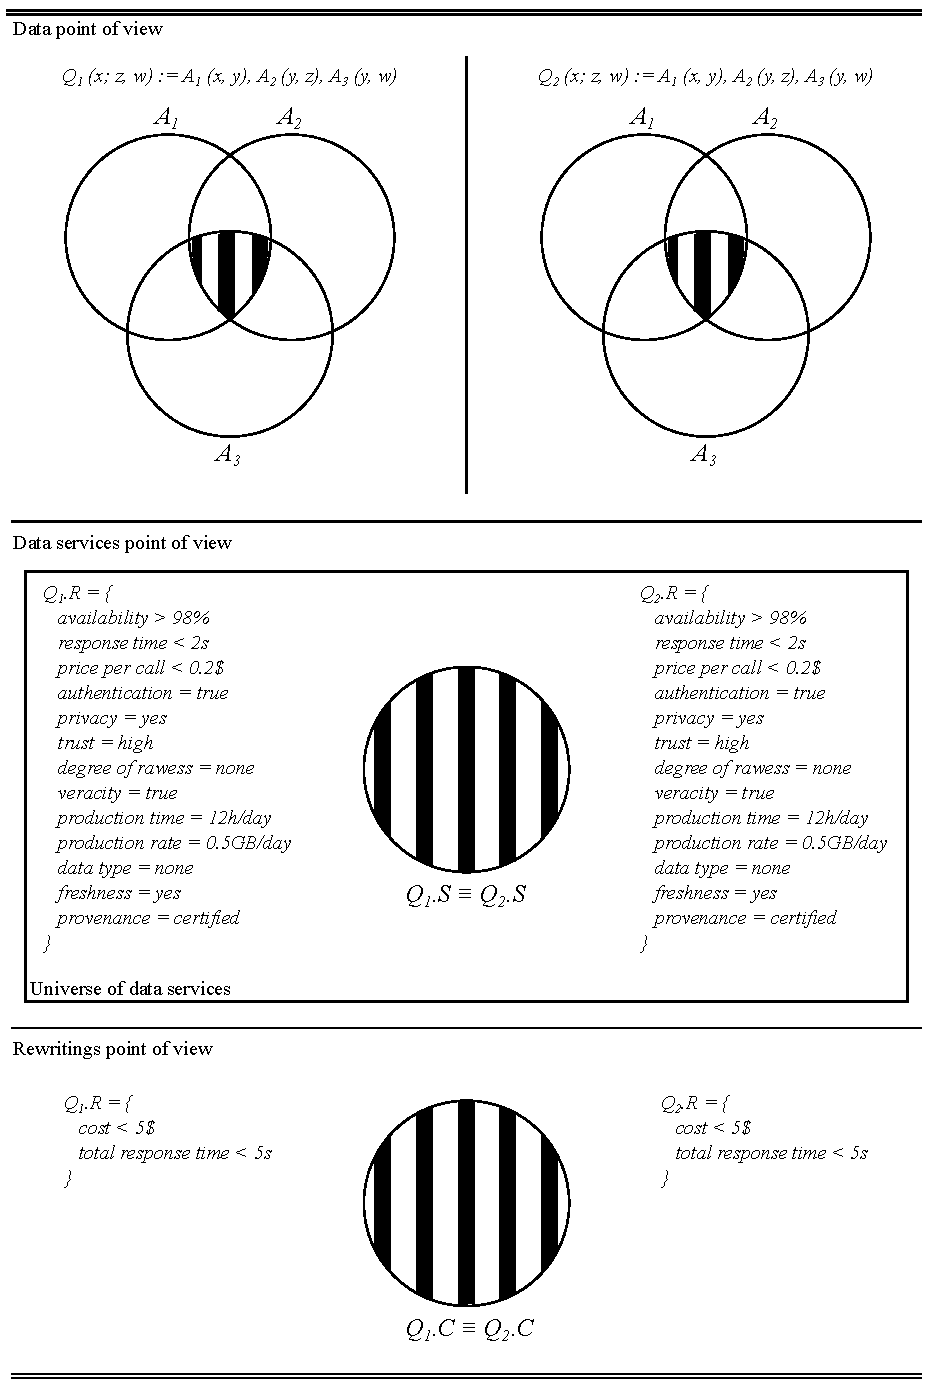
\includegraphics[scale=0.9]{images/QT1.pdf}
\caption{Query type 1 representation.}
\label{fig:qt1}
\end{figure}

\begin{definition}\label{def:reqeq}
A set of \textsl{user requirements} $R_{1}$ is equivalent to a set of \textsl{user requirements} $R_{2}$, represented by $R_{1} \equiv R_{2}$, if and only if: $\forall r_{i} \in R_{1}, \ \exists r_{j} \in R_{2} \ \vert \ eval (r_{i}) = eval(r_{j}) \ and \ \vert R_{1} \vert = \vert R_{2} \vert$.
\end{definition}

\begin{definition}\label{def:qt1}
Query Type 1 -- a query $Q_{1}$ is equivalent to a query $Q_{2}$, if and only if: $Q_{1}.A = Q_{2}.A$ and $Q_{1}.R_{1} \equiv Q_{2}.R_{2}$.
\end{definition}

From the re-usability point of view, everything from $Q_{1}$ could be reused to answer $Q_{2}$. All data services filtered to the query $Q_{1}$, denoted $Q_{1}.S$, potentially could be reused in the query $Q_{2}$, excepting the ones that are not online in the exact moment. 
The set of compositions produced to the query $Q_{1}$, denoted as $Q_{1}.C$, potentially could be used to answer the query $Q_{2}$, excepting the ones using offline data services. Following, the reusability function for data services, rewritings and queries are presented. 

The service reusability function, denoted as $reuse \ services(<query>, <query \ type>)$, receives as parameters a query and a query type, and returns a set of reusable data services.

\begin{definition}\label{def:rsqt1}
Given $Q_{1}$ and $Q_{2}$, queries of type 1, the reusability of services $reuse \ services(Q_{1}, type \ 1)$ selects and returns all data services in $Q_{1}.S$ online in the exact moment. 
\begin{center}
$Q_{2}.S = Q_{2}.S \ \cup \ \lbrace ds_{i} \rbrace, \ \forall ds_{i} \in Q_{1}.S \ \vert \ ds_{i} \ is \ online$.
\end{center}
\end{definition}

The rewritings reusability function, denoted as $reuse \ rewritings(<query>, <query>)$, receives as parameters a previous query and the new query, and returns a set of reusable rewritings to answer the last one.

\begin{definition}\label{def:rrqt1}
Given $Q_{1}$ and $Q_{2}$, queries of type 1, the reusability of rewritings $reuse \ rewritings(Q_{1}, \ Q_{2})$ selects and returns all rewritings in $Q_{1}.C$ which uses the services in $Q_{2}.S$. 
\begin{center}
$Q_{2}.C = Q_{2}.C \ \cup \ \lbrace c_{i} \rbrace, \ \forall c_{i} \in Q_{1}.C \ \vert \
   \lbrace \ \forall ds_{j} \in c_{i}, \ \nexists ds_{k} \in c_{i} \ \vert \ ds_{j} \in Q_{2}.S \ and \ ds_{k} \notin Q_{2}.S \rbrace$.
\end{center}
\end{definition}

\begin{enumerate}[b)]
\item \textcolor{red}{Continuar aqui..query less restrict} \textit{Query type 1:} the \textit{first} type is the simplest case. The figure~\ref{fig:qt1} illustrates the manner this query is represented. Given a previous query $Q_{1}$ and an incoming query $Q_{2}$, $Q_{1}$ is equivalent to $Q_{2}$ when: \textit{(1)} both queries expect the same data as answer, which means they cover the same abstract services (Figure~\ref{fig:qt1} - Data point of view). In this sense, the set of abstract service of $Q_{1}$, denoted as $Q_{1}.A$, is equals to the set of abstract services of $Q_{2}$, denoted as $Q_{2}.A$.
%
\begin{center}
$Q_{1}.A = Q_{2}.A$
\end{center}
%
\textit{(2)} For each user requirement $r_{i}$ in $Q_{1}.R$, there is a user requirement $r_{j}$ in $Q_{2}.R$ such that the evaluation of $r_{i}$ is equal to the evaluation of $r_{j}$. 
Consequently, the score of $Q_{1}.R$ is equals to the score of $Q_{2}.R$. The \textit{query type 1} and the equivalence between requirements are formally defined below.
\end{enumerate}


\subsubsection{Query type 2: $Q_{2}$ is a subset of $Q_{1}$}

The \textit{second} type deals with \textit{query subsets} due to more restrict user requirements. Given two queries $Q_{1}$ and $Q_{2}$, $Q_{2}$ is a subset of $Q_{1}$ when:
%
\begin{enumerate}[a)]
\item They expect the same data as answer, which means they cover the same abstract services. 
For instance, the set of abstract service of $Q_{1}$, denoted as $Q_{1}.A$, is equals to the set of abstract services of $Q_{2}$, denoted as $Q_{2}.A$.
%
\begin{center}
$Q_{1}.A = Q_{2}.A$
\end{center}
%
\item For all user requirement $r_{i}$ in $Q_{2}.R$, there is at least one $r_{j}$ in $Q_{1}.R$ such that the evaluation of $r_{i}$ is contained in the evaluation of $r_{j}$. 
For all $r_{k}$ in $Q_{2}.R$, there is no $r_{l}$ in $Q_{1}.R$ such that the evaluation of $r_{l}$ is contained in the evaluation of $r_{k}$. 
Consequently, the score of $Q_{1}.R$ is lower than the score of $Q_{2}.R$. The definition of more restrict requirements is presented below.
\end{enumerate}

\begin{definition}\label{def:reqmore}
Given a set of \textsl{user requirements} $R_{1}$ and $R_{2}$, $R_{1}$ is more restrict than $R_{2}$, represented by $R_{1} \ \rhd \ R_{2}$, if and only if: $\forall r_{i} \in R_{1}, \ \exists r_{j} \in R_{2}, \ \nexists r_{k} \in R_{2} \ \vert \ eval (r_{i}) \subset eval(r_{j}) \ and \ eval (r_{k}) \subset eval(r_{i}) \ and \ \vert R_{1} \vert = \vert R_{2} \vert$.
\end{definition}

From the re-usability point of view, a subset of the data services filtered to the query $Q_{1}$ which are \textit{online} in the moment, $online(Q_{1}.S)$, could be reused in the query $Q_{2}$. This fact occurs due to the more restrict requirements imposed by $Q_{2}$.
With respect to the compositions, a subset of the rewritings produced to the query $Q_{1}$ could also be used to answer the query $Q_{2}$. These rewritings should use the data services in $online(Q_{1}.S)$, denoted as $available(Q_{1}.C)$, and respect the more restrict requirements defined in $Q_{2}$. 
The query type 2 definition is presented below.

\begin{definition}\label{def:qt2}
Query Type 2 -- a query $Q_{1}$ is a subset of a query $Q_{2}$, if and only if: $Q_{1}.A = Q_{2}.A$ and $Q_{1}.R_{1} \rhd Q_{2}.R_{2}$
\end{definition}
